\chapter{水声传感网络MAC协议仿真}
\section {仿真软件介绍}
\subsection{NS2}
NS2(Network Simulator,version 2)是一种面向对象的网络仿真器,本质上是一个离散事件模拟器,由UC Berkeley开发而成。它本身有一个虚拟时钟,所有的仿真都由离散事件驱动的。
NS2使用C++和Otcl作为开发语言。它包含仿真事件调度器、网络组件对象库以及网络构建模型库等。事件调度器计算仿真时间,并且激活事件队列中的当前事件,执行一些相关的事件,网络组件通过传递分组来相互通信,但这并不耗费仿真时间。所有需要花费仿真时间来处理分组的网络组件都必须要使用事件调度器。它先为这个分组发出一个事件,然后等待这个事件被调度回来之后,才能做下一步的处理工作。事件调度器的另一个用处就是计时。
CBR,以确定的速率产生通信量,分组尺寸固定,可在分组间隔之间产生随机抖动。
\subsection{Aqua-Sim}
美国康涅狄格州大学的水下无线通迅网络研究所在NS2的基础上扩展了专门用于水下环境的仿真平台Aqua-Sim。它可以十分逼真地仿真水声信道,对信号衰减和水下包碰撞的仿真十分有效。同时它也实现了一套完整的从物理层到应用层的协议栈,各层之间可以独立发展。
 
 Object Oriented Design: htextensible and flexible
 Open Architecture: easily import new protocols
 
 \begin{figure}[ht]
 	\centering
 	\includegraphics[scale=0.5]{figures/aq.png}
 	\caption{
 		水声传感网络
 	}
 	\label{fig:example}
 \end{figure}
\subsubsection{衰减模型}
根据f l=3km k=2 Pt 30w吸收系数
\begin{equation}
\alpha=\frac{0.11f^2}{1+f^2}+\frac{44f^2}{4100+f^2}+3.0*10^{-4}f^2+3.3*10^{-3}
\end{equation}
传播损失
\begin{equation}
A(l,f)=l^k\times(10^{\frac{\alpha (f)}{10}})^l
\end{equation}

\begin{equation}
TxThresh=\frac{Pt}{A(l,f)}
\end{equation}

\subsubsection{能量模型}
根据节点传输状态IDLE,SEND,RECV分别调用函数
void EnergyModel::DecrIdleEnergy(double idletime, double P\_idle)
void EnergyModel::DecrRcvEnergy(double rcvtime, double P\_rcv)
void EnergyModel::DecrTxEnergy(double txtime, double P\_tx)
将节点不同状态下的功率乘以状态持续时间,计算出总的能耗。

\subsubsection{碰撞模型}
节点接收数据时,如果节点正处于接收状态,计算到达数据包的能量和正在接收数据包的能量之比。
\begin{equation}
\begin{aligned}
&if \ \ \  \frac{Pr_{\mbox{到达}}}{Pr_{\mbox{接收}}}\  >CPThresh\\
&\ \ \ \ \ \ capture(\mbox{到达数据包});\\
&else\\
&\ \ \ \ \ \ discard(\mbox{到达数据包});
\end{aligned}
\end{equation}

\section {场景和参数设置}
 \begin{figure}[ht]
 	\centering
 	\includegraphics[scale=0.5]{figures/2scen.png}
 	\caption{
 		水声传感网络
 	}
 	\label{fig:example}
 \end{figure}
 
  \begin{figure}[ht]
  	\centering
  	\includegraphics[scale=0.5]{figures/3scen.png}
  	\caption{
  		水声传感网络
  	}
  	\label{fig:example}
  \end{figure}
  
\begin{table}[!htp]
	\centering
\caption{仿真场景及参数设置}
\begin{tabular}{|c|c|}% 通过添加 | 来表示是否需要绘制竖线
	\hline  % 在表格最上方绘制横线
	\multicolumn{2}{|c|}{仿真场景及参数设置}\\
	\hline  %在第一行和第二行之间绘制横线
	固定节点数& 12\\
	\hline
	移动节点数& 2\\
	\hline
	移动节点运动速度& 2.5m/s\\
	\hline
	节点通信半径& 3000m\\
	\hline
	相邻固定节点距离& 2000m\\
	\hline
	仿真时间数& 2400s\\
	\hline
	频率& 10kHz\\
	\hline				
	节点传输速率& 1kbps\\
	\hline
	数据包大小& 300Bytes\\
	\hline
	节点发送报文功率& 30w\\
	\hline				
	节点接收报文功率& 1w\\
	\hline
	节点侦听报文功率& 0.2w\\	
	\hline	
\end{tabular}
\label{tab2}
\end{table}

\section {仿真结果与分析}
\subsection{理论曲线(低负载 高负载)}
\begin{figure}[!ht]
	\centering
	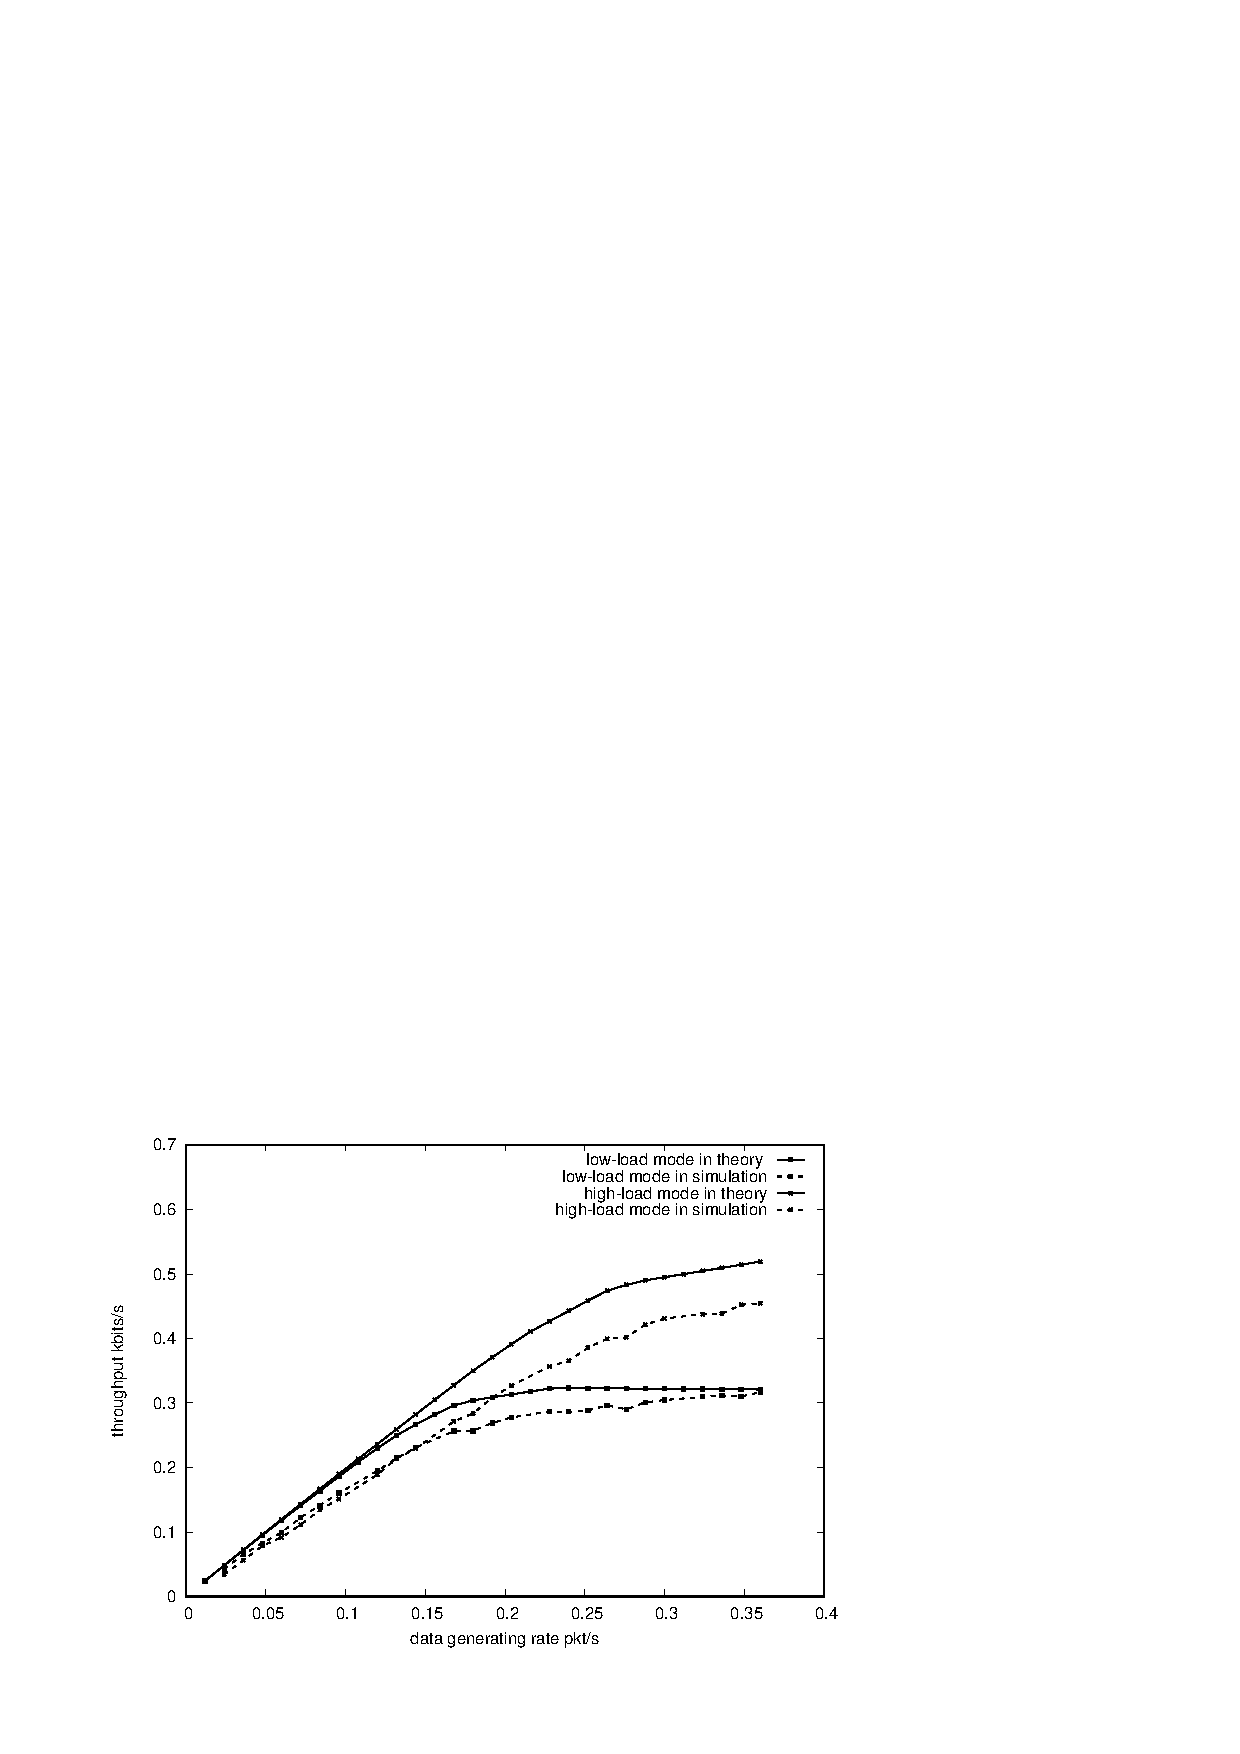
\includegraphics[scale=0.8]{figures/lilun.pdf}
	\caption{
		水声传感网络
	}
	\label{fig:example}
\end{figure}
\subsection{性能指标}
 在处理相同数据流的情况下,判断不同MAC协议下网络性能的好坏。判断网络性能时,主要统计四个网络数据指标,网络的平均时延、网络的平均吞吐量、网络的能耗、网络的数据包发送成功率。
 (1)网络的平均时延是指数据包从源节点到达目的节点在网络中的传播时间。网络的时延=数据包的发送时延+数据包的传输时延+数据包的接收时延。 
 (2)网络吞吐量表示网络成功发送的数据包数。网络的平均吞吐量定义为吞吐量主要用于衡量网络利用率和网络数据最大容量。
 (3)网络的能耗定义为网络中的所有节点在整个网络运行期间所消耗的总的能量,即为网络初始化时的总能量减去网络仿真结束时剩余的能量。
 (4)网络的数据包发送成功率是指网络中正确接收到的数据包数和总的发送数据包数的比值。
\subsection{结果分析}


\begin{figure}[!ht]
	\centering
	\includegraphics[scale=0.8]{figures/2nodea.pdf}
	\caption{
		水声传感网络
	}
	\label{fig:example}
\end{figure}

\begin{figure}[!ht]
	\centering
	\includegraphics[scale=0.8]{figures/2nodeb.pdf}
	\caption{
		水声传感网络
	}
	\label{fig:example}
\end{figure}

\begin{figure}[!ht]
	\centering
	\includegraphics[scale=0.8]{figures/2nodec.pdf}
	\caption{
		水声传感网络
	}
	\label{fig:example}
\end{figure}

\begin{figure}[!ht]
	\centering
	\includegraphics[scale=0.8]{figures/2noded.pdf}
	\caption{
		水声传感网络
	}
	\label{fig:example}
\end{figure}


\begin{figure}[!ht]
	\centering
	\includegraphics[scale=0.8]{figures/3nodea.pdf}
	\caption{
		水声传感网络
	}
	\label{fig:example}
\end{figure}

\begin{figure}[!ht]
	\centering
	\includegraphics[scale=0.8]{figures/3nodeb.pdf}
	\caption{
		水声传感网络
	}
	\label{fig:example}
\end{figure}

\begin{figure}[!ht]
	\centering
	\includegraphics[scale=0.8]{figures/3nodec.pdf}
	\caption{
		水声传感网络
	}
	\label{fig:example}
\end{figure}

\begin{figure}[!ht]
	\centering
	\includegraphics[scale=0.8]{figures/3noded.pdf}
	\caption{
		水声传感网络
	}
	\label{fig:example}
\end{figure}

\endinput